\documentclass[12pt]{article}

\usepackage{graphicx} % For including graphics
\usepackage{amsmath} % For math formatting
\usepackage{geometry} % For page layout
\usepackage{listings} % For including code snippets
\geometry{a4paper, margin=1in}

\title{Chaotic Dynamics - Chua's Circuit}
\author{Enrique Rivera Jr. \\
                Physics Undergraduate, \\ 
                The University of Texas at Austin}
\date{\today}

\begin{document}
\maketitle

\begin{abstract}
        valuable insights into the behavior of complex systems.
\end{abstract}

\section{Introduction}
        \subsection{Background and Theory}

                \subsubsection{Chaos Theory} 
                Chaos theory is a branch of mathematics and physics that studies complex systems that exhibit 
                sensitive dependence on initial conditions. One of the key concepts in chaos theory is the butterfly
                 effect, which states that small changes in the initial conditions of a system can lead to large and 
                 unpredictable differences in the long-term behavior of the system. This phenomenon highlights the inherent 
                 difficulty in making long-term predictions for chaotic systems.

                Another important aspect of chaos theory is the presence of autonomous variables. These variables are 
                self-governing and evolve according to their own internal dynamics, often leading to complex and unpredictable 
                behavior. In the context of this paper, we will explore the chaotic dynamics of Chua's circuit, which is known 
                for its rich and intricate behavior.

                Understanding chaos theory and its implications for long-term prediction is crucial in various scientific 
                fields, including physics, biology, economics, and weather forecasting. By studying chaotic systems, 
                researchers aim to uncover underlying patterns and develop mathematical models that can capture their behavior.

                In the context of chaos theory, autonomous variables refer to variables that evolve according to their own i
                nternal dynamics, independent of external influences. These variables can exhibit complex and unpredictable 
                behavior, contributing to the overall chaotic dynamics of a system.

                Autonomous variables are often associated with the presence of strange attractors in chaotic systems. 
                An attractor is a set of values or states towards which a system tends to evolve over time. In chaotic 
                systems, attractors can take on complex and irregular shapes, known as strange attractors. These strange 
                attractors are characterized by their fractal nature, meaning they exhibit self-similarity at different scales.

                Attractor points, also known as fixed points or equilibrium points, are specific states within an attractor where 
                the system remains unchanged over time. These points represent stable or unstable states of the system. Stable 
                attractor points are like valleys in the system's behavior, where nearby states tend to converge towards the 
                point. Unstable attractor points, on the other hand, are like hills, where nearby states tend to diverge away 
                from the point.

                In the case of Chua's circuit, the behavior of the system is governed by the interplay of the capacitor, 
                inductor, and nonlinear resistor. The presence of autonomous variables and strange attractors in Chua's circuit 
                leads to its chaotic dynamics. The system can exhibit complex and unpredictable behavior, with attractor points 
                representing stable or unstable states towards which the system tends to evolve


                \subsubsection{Chua's Circuit}

                Chua's circuit is a simple electronic circuit that exhibits chaotic behavior. The circuit consists of
                three basic components: a capacitor, an inductor, and a nonlinear resistor. The nonlinear resistor 
                is the key element that introduces chaotic dynamics into the system. The behavior of Chua's circuit 
                is described by a set of nonlinear differential equations, which can give rise to complex and unpredictable 
                behavior under certain conditions.

                Chua's circuit is an example of a dynamical system, which is a system that evolves over time according to
                a set of rules or equations. In the case of Chua's circuit, the behavior of the system is governed by the
                interplay of the three basic components, as well as the nonlinear dynamics introduced by the resistor.

                The study of Chua's circuit and its chaotic behavior has important implications for the field of nonlinear
                dynamics and chaos theory. By understanding the behavior of Chua's circuit, researchers can gain insights
                into the underlying principles of chaotic systems and develop mathematical models that capture their behavior.

                The Chua's circuit is a simple electronic circuit that exhibits chaotic behavior. The circuit consists of
                three basic components: a capacitor, an inductor, and a nonlinear resistor. The nonlinear resistor is the
                key element that introduces chaotic dynamics into the system. The behavior of Chua's circuit is described
                by a set of nonlinear differential equations, which can give rise to complex and unpredictable behavior.

                The capacitor and the indcutor create the base oscillation of the circuit. As we'll see when in the oscilloscope,
                the capacitor and inductor create a sinusoidal wave. Then with the poteniometers, we can change the variables of the 
                system and see how the phase space changes.


        \subsection{Purpose}
                The purpose of this experiment is to empirically confirm the theoretical projections of chaotic dynamics and 
                explore the boundaries of classical mechanics under high-energy conditions. By studying the behavior of Chua's 
                circuit and its chaotic dynamics, we aim to gain insights into the complex and unpredictable behavior of 
                autonomous systems. Additionally, we seek to explore the presence of strange attractors and fractal patterns 
                in the behavior of Chua's circuit.

\section{Experimental Setup and Procedure}
        \subsection{Apparatus}
                \subsubsection{Equipment}
                For this experiment, we used the following equipment: Oscilloscope, Multimeter, Function Generator, and a Chua's Circuit that used Breadboard,
                Resistors, Capacitors, Inductor, and Chua diode. The oscilloscope was used to visualize the behavior of the Chua's circuit, 
                while the multimeter was used to measure the resistance and capacitance of the components. The function generator was used to 
                provide the input signal to the Chua's circuit, and the Chua's circuit itself was used to study the chaotic dynamics of the system.
                        
                \subsubsection{Schematic}
                
                \begin{figure}[h!]
                        \centering
                        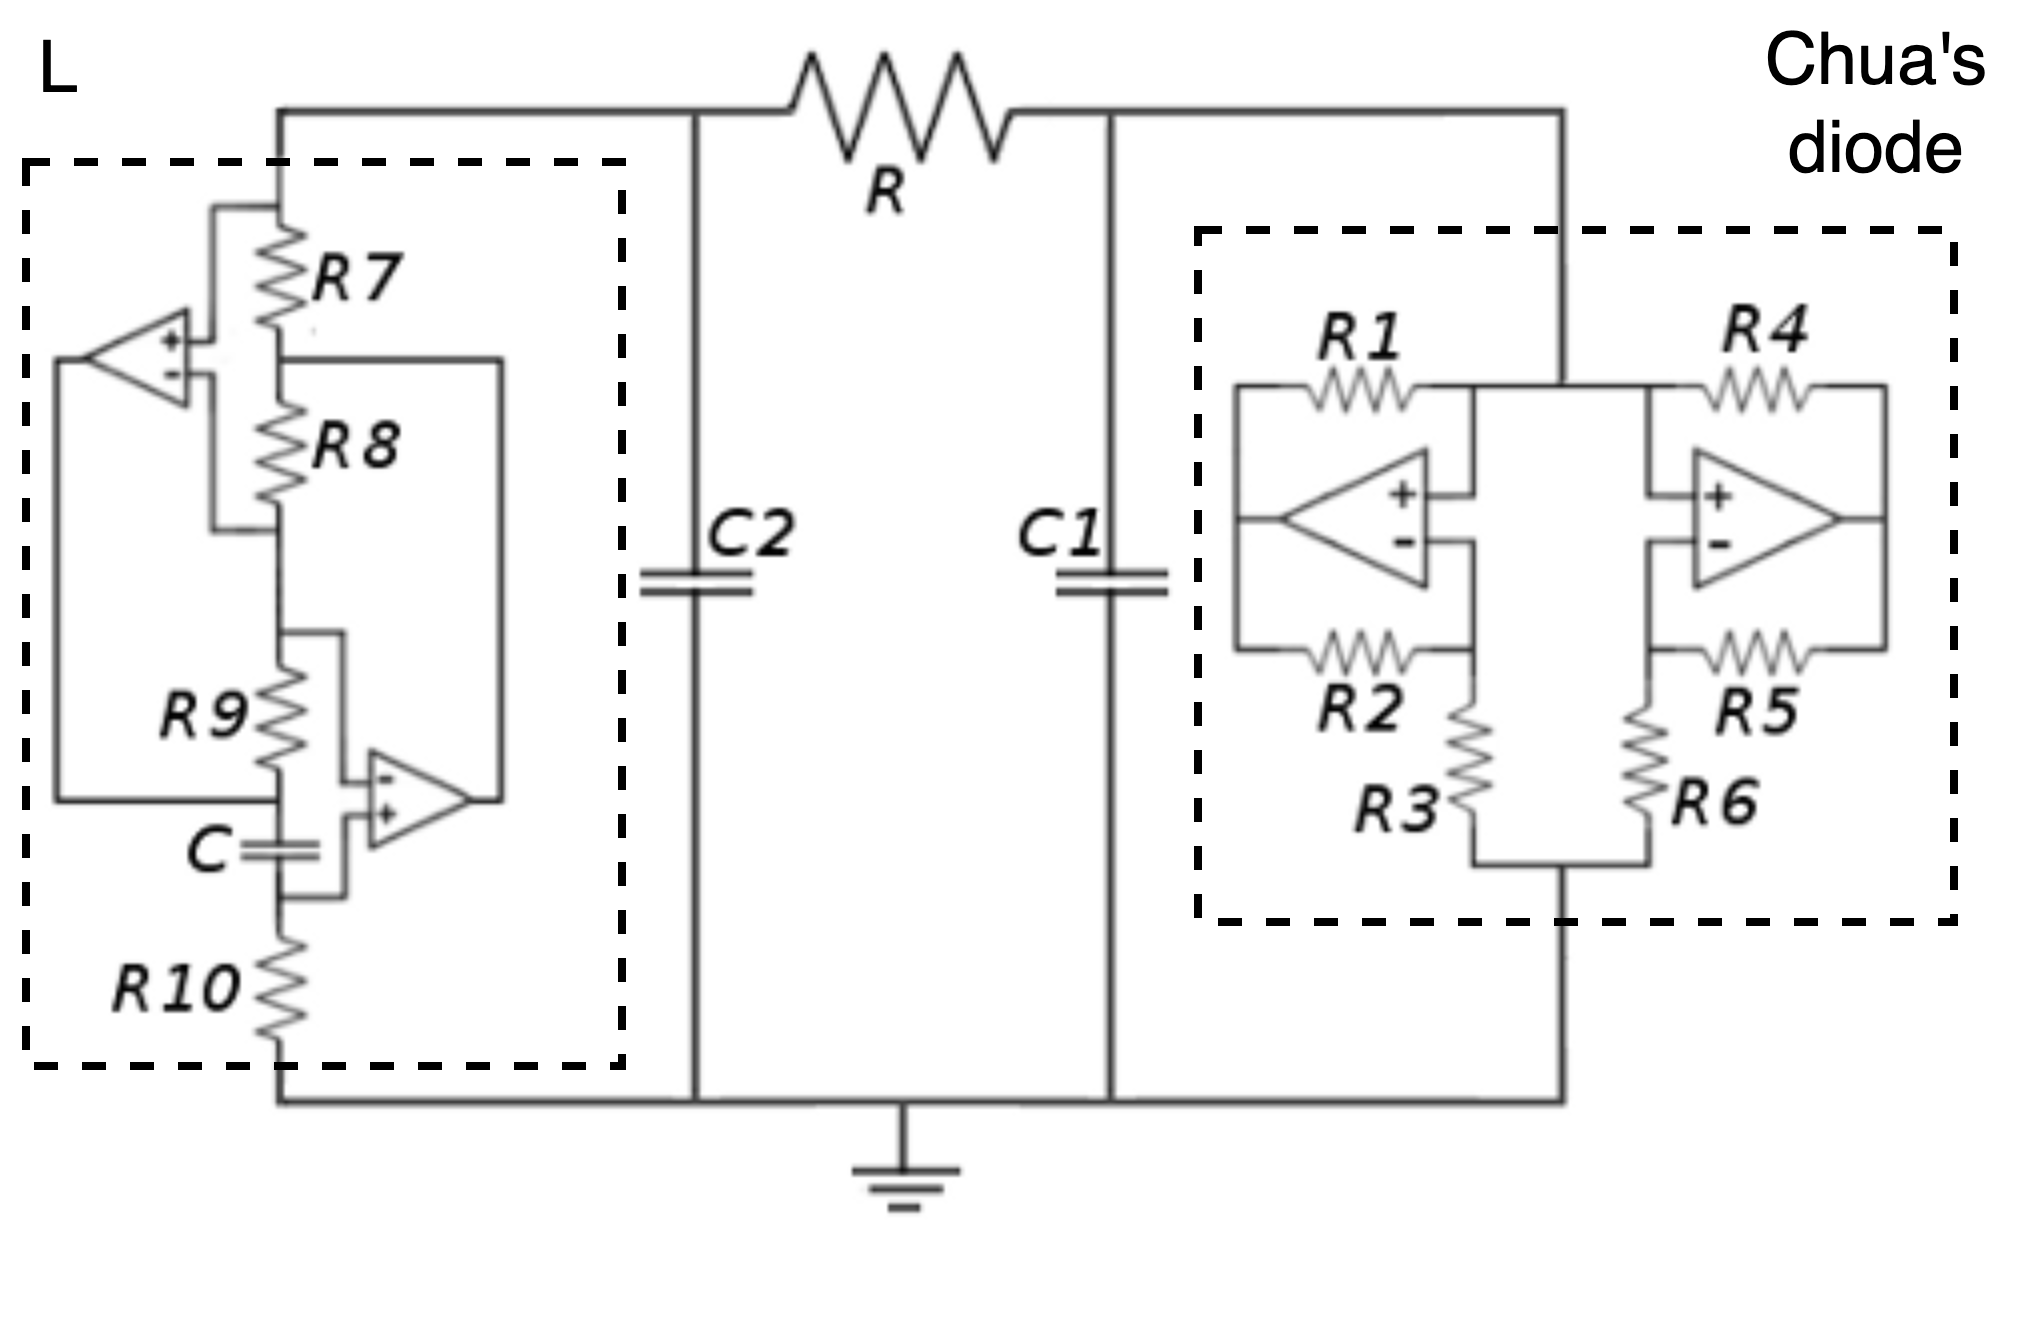
\includegraphics[width=0.7\textwidth]{./img/other/circuit_img.png}
                        \caption{Circuit Diagram of Chua's Circuit. In the figure, we have the schematic of the Chua's circuit. We can see the three basic components: a capacitors(in the center), 
                        an inductor(on the left, denoted with L), and a nonlinear resistor(on the right, the Chua'a diode). The nonlinear resistor is the key element that introduces chaotic dynamics into the system.}
                        \label{fig: Circuit Diagram of Chua's Circuit.}
                \end{figure}

                
                \begin{table}[ht]
                        \centering
                        \begin{tabular}{|c|c|}
                                \hline
                                Component & Value \\
                                \hline
                                R & 10k $\Omega$ (pot.)\\
                                R1 & 220 $\Omega$ \\
                                R2 & 220 $\Omega$ \\
                                R3 & 2.2 k$\Omega$\\
                                R4 & 22.0 k$\Omega$ \\
                                R5 & 22.0 k$\Omega$ \\
                                R6 & 3.3 k$\Omega$ \\
                                R7 & 100 $\Omega$ \\
                                R8 & 1.0 k$\Omega$ \\
                                R9 & 1.0 k$\Omega$ \\
                                R10 & 10k$\Omega$ (pot.) \\
                                C1 & 10 nF \\
                                C2 & 100 nF \\
                                L & 15 mH \\
                                \hline
                        \end{tabular}
                        \caption{Values of the components used in the Chua's Circuit. In the table, we have the values of the 
                        components used in the Chua's circuit. We can see the values of the resistors, capacitors, and inductor.}
                        \label{tab: Values of the components used in the Chua's Circuit.}
                \end{table}
                        

                

\section{Results}
        \subsection{Data and Analysis}

        For the data and analysis, we used the oscilloscope to visualize the behavior of the Chua's circuit. 
        We varied the initial conditions of the circuit by adjusting the potentiometers and observed the resulting behavior. 
        We also used the oscilloscope to measure the voltage across the capacitors. 
        The data collected from the oscilloscope was then exported and analyzed to identify the presence of strange attractors and fractal patterns 
        in the behavior of the Chua's circuit. There where about 5 succesful trials, and the data was analyzed using the python library matplotlib.

        \begin{figure}[!htb]
                \centering
                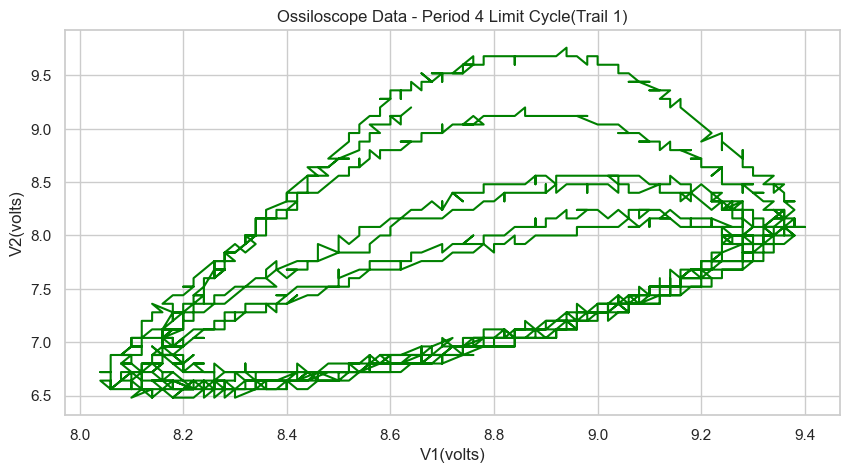
\includegraphics[width=0.7\textwidth]{./img/plots/Trail1_VonV.png}
                \caption{Trail 1 - V1 vs V2. In the figure, we have the plot of the voltage on the capacitor 1 versus the voltage on the capacitor 2. 
                We can see the chaotic behavior of the system. The plot shows the presence of strange attractors and fractal patterns, and this one specifically shows a period 4 cycle.}
                \label{fig: Trail 1 - V on V.}
        \end{figure} \pagebreak
        \begin{figure}[!htb]
                \centering
                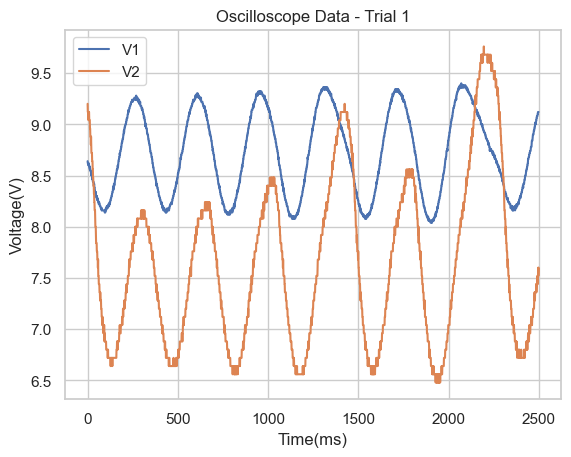
\includegraphics[width=0.7\textwidth]{./img/plots/Trail1_O.png}
                \caption{Trail 1 - V1 and V2 vs time. In the figure, we have the plot of the voltage on the capacitor 1 and the voltage on the capacitor 2 versus time. 
                Here we can see the sinusoidal behavior of the system. }
        \end{figure}


        \begin{figure}[!htb]
                \centering
                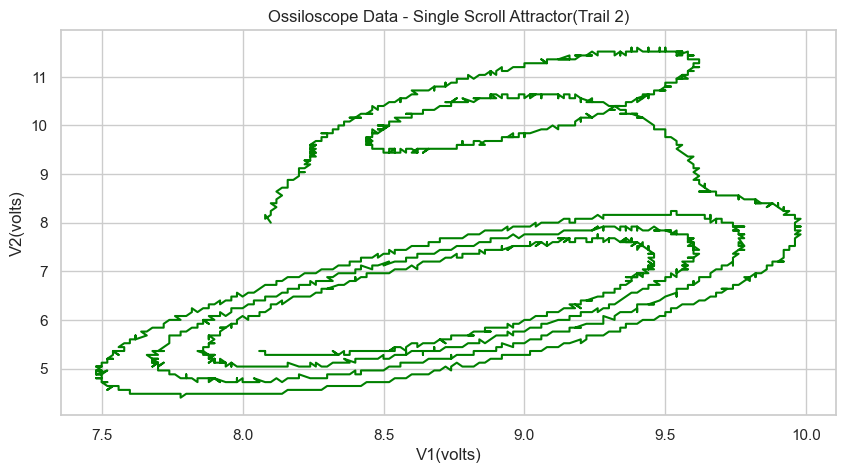
\includegraphics[width=0.7\textwidth]{./img/plots/Trial2_VonV.png}
                \caption{Trail 2 - V1 vs V2. In the figure, we have the plot of the voltage on the capacitor 1 versus the voltage on the capacitor 2. 
                We can see the chaotic behavior of the system. The plot shows the presence of strange attractors and fractal patterns, and this one specifically single scroll attractor.}
                \label{fig: Trail 2 - V on V.}
        \end{figure} \pagebreak
        \begin{figure}[!htb]
                \centering
                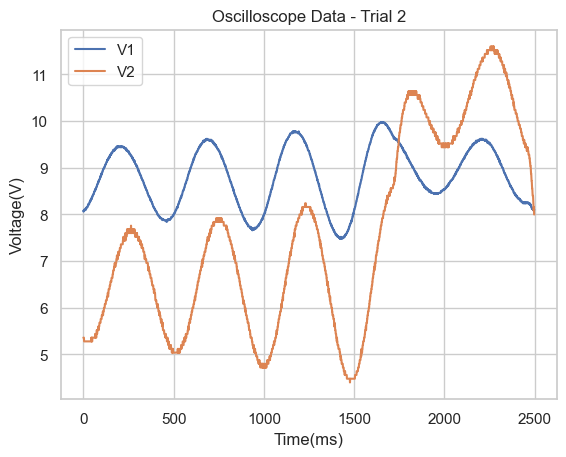
\includegraphics[width=0.7\textwidth]{./img/plots/Trail2_O.png}
                \caption{Trail 2 - V1 and V2 vs time. In the figure, we have the plot of the voltage on the capacitor 1 and the voltage on the capacitor 2 versus time. 
                Here we can see the sinusoidal behavior of the system. }
        \end{figure}


        \begin{figure}[!htb]
                \centering
                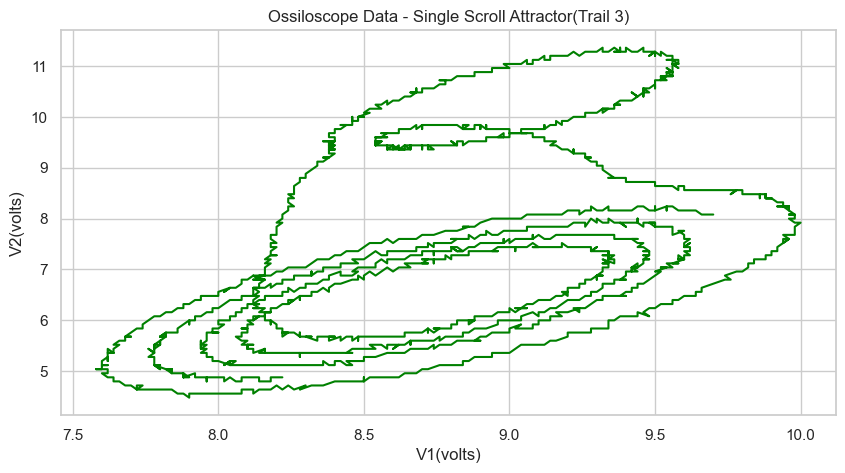
\includegraphics[width=0.7\textwidth]{./img/plots/Trail3_VonV.png}
                \caption{Trail 3 - V1 vs V2. In the figure, we have the plot of the voltage on the capacitor 1 versus the voltage on the capacitor 2. 
                We can see the chaotic behavior of the system. The plot shows the presence of strange attractors and fractal patterns, and this one specifically shows a singal scroll attractor}
                \label{fig: Trail 3 - V on V.}
        \end{figure} \pagebreak
        \begin{figure}[!htb]
                \centering
                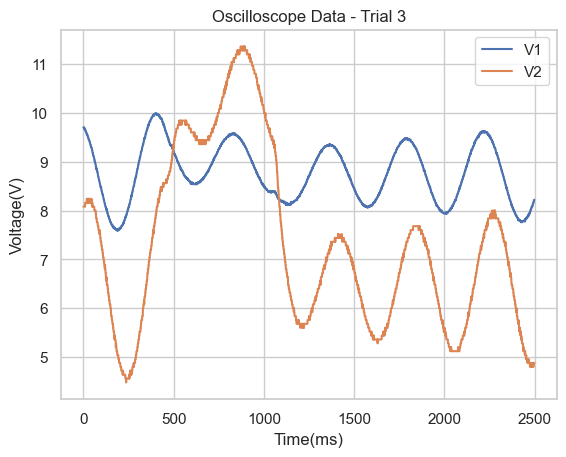
\includegraphics[width=0.7\textwidth]{./img/plots/Trail3_O.png}
                \caption{Trail 3 - V1 and V2 vs time. In the figure, we have the plot of the voltage on the capacitor 1 and the voltage on the capacitor 2 versus time. 
                Here we can see the sinusoidal behavior of the system. }
        \end{figure}


        \begin{figure}[h!]
                \centering
                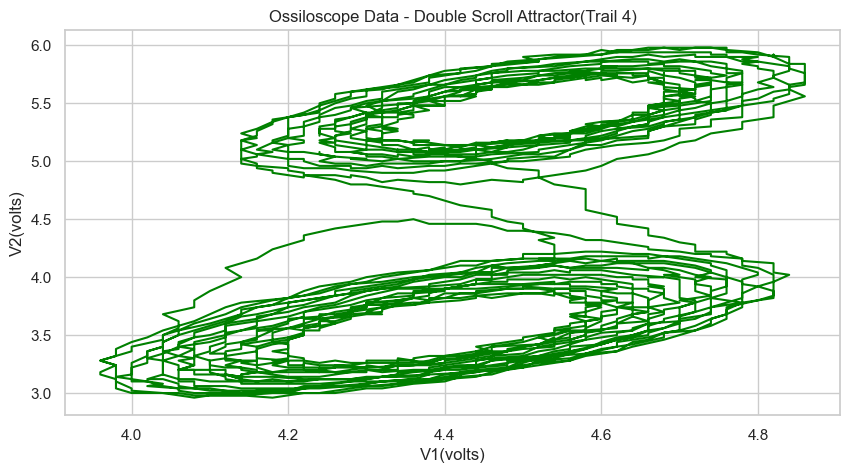
\includegraphics[width=0.7\textwidth]{./img/plots/Trail4_VonV.png}
                \caption{Trail 4 - V1 vs V2. In the figure, we have the plot of the voltage on the capacitor 1 versus the voltage on the capacitor 2. 
                We can see the chaotic behavior of the system. The plot shows the presence of strange attractors and fractal patterns, and this one specifically shows a double scroll attractor.}
                \label{fig: Trail 4 - V on V.}
        \end{figure} \pagebreak
        \begin{figure}[h!]
                \centering
                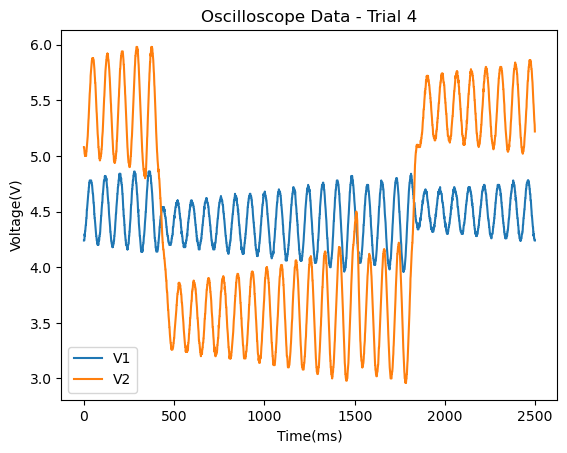
\includegraphics[width=0.7\textwidth]{./img/plots/Trail4_O.png}
                \caption{Trail 4 - V1 and V2 vs time. In the figure, we have the plot of the voltage on the capacitor 1 and the voltage on the capacitor 2 versus time. 
                Here we can see the sinusoidal behavior of the system. }
        \end{figure}


        \begin{figure}[h!]
                \centering
                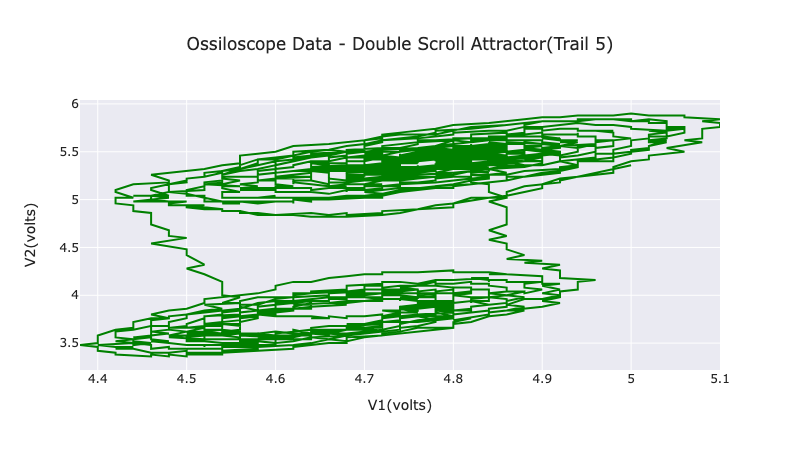
\includegraphics[width=0.7\textwidth]{./img/plots/Trail5_VonV.png}
                \caption{Trail 5 - V1 vs V2. In the figure, we have the plot of the voltage on the capacitor 1 versus the voltage on the capacitor 2. 
                We can see the chaotic behavior of the system. The plot shows the presence of strange attractors and fractal patterns, and this one specifically shows a double scroll attractor}
                \label{fig: Trail 5 - V on V.}
        \end{figure} \pagebreak
        \begin{figure}[h!]
                \centering
                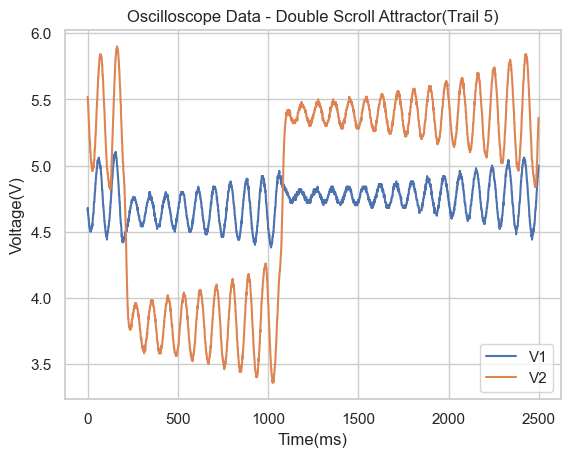
\includegraphics[width=0.7\textwidth]{./img/plots/Trail5_O.png}
                \caption{Trail 5 - V1 and V2 vs time. In the figure, we have the plot of the voltage on the capacitor 1 and the voltage on the capacitor 2 versus time. 
                Here we can see the sinusoidal behavior of the system. }
        \end{figure}
        \subsection{Chua's Circuit Behavior}
                \subsubsection{Initial Conditions}
                The behavior of Chua's circuit is highly sensitive to initial conditions. Small changes in the initial conditions
                can lead to large and unpredictable differences in the long-term behavior of the system. This sensitivity to initial
                conditions is a hallmark of chaotic systems and is known as the butterfly effect.

                We can see the chaotic behavior of the system in the plots of the voltage on the capacitor 1 versus the voltage on the
                capacitor 2. The plots show the presence of strange attractors and fractal patterns, which are characteristic of chaotic
                systems. The behavior of the system is highly sensitive to initial conditions, and small changes in the potentiometers
                can lead to large and unpredictable differences in the long-term behavior of the system. This was done by changing the voltage 
                feeding the circuit, and the resistance of the potentiometers.

                \subsubsection{Strange Attractors}
                As we can see in the plots, the presence of strange attractors is evident in the behavior of Chua's circuit. Strange
                attractors are characterized by their complex and irregular shapes, which exhibit self-similarity at different scales.
                The presence of strange attractors in the behavior of Chua's circuit is a key feature of chaotic systems and highlights
                the complex and unpredictable behavior of the system.
                
                These attractor points represent stable or unstable states of the system. Stable attractor points are like valleys in the
                system's behavior, where nearby states tend to converge towards the point. Unstable attractor points, on the other hand,
                are like hills, where nearby states tend to diverge away from the point.

                However, from the graphs we only see a single scroll attractor, and a double scroll attractor. This means at most the system had 
                two attractor points with the Tail 5 having a double scroll attractor. This is often called a strange attractor. From trail 1 we 
                can see the base oscillations of the system, and from the other trails we can see the chaotic behavior of the system.
                
                \begin{equation}
                        \frac{dv_1}{dt} = \frac{1}{C_1} (G(v_2 - v_1) - g(v_1)),
                        \end{equation}
                        \begin{equation}
                        \frac{dv_2}{dt} = \frac{1}{C_2} (G(v_1 - v_2) + i_L),
                        \end{equation}
                        \begin{equation}
                        \frac{di_L}{dt} = \frac{1}{L} (-v_2 - R_0i_L),
                        \end{equation}
                
                where $v_1$ and $v_2$ are the voltages across the capacitors, $i_L$ is the current across the inductor, $C_1$ and $C_2$ are the capacitances of the capacitors, $L$ is the inductance of the inductor, $R_0$ is the resistance of the inductor, $G$ is the conductance of the negative resistance, and $g(v_1)$ is the nonlinear function of the voltage across the capacitor 1. The nonlinear function $g(v_1)$ is given by:
                \[
                g(v_R) = 
                \begin{cases}
                G_bv_R + (G_b - G_a)E_1, & \text{if } v_R \leq -E_1, \\
                G_av_R, & \text{if } \lvert v_R \rvert < E_1, \\
                G_bv_R + (G_a - G_b)E_1, & \text{if } v_R \geq E_1.
                \end{cases}
                \]
                where $G_a$, $G_b$, and $E_1$ are constants that determine the shape of the nonlinear function. The nonlinear function $g(v_1)$ is the key element that introduces chaotic dynamics into the system, and its shape determines the behavior of the system. The presence of autonomous variables and strange attractors in the behavior of Chua's circuit leads to its chaotic dynamics. The system can exhibit complex and unpredictable behavior, with attractor points representing stable or unstable states towards which the system tends to evolve.

                        
                \begin{figure}[!htb]
                        \centering
                        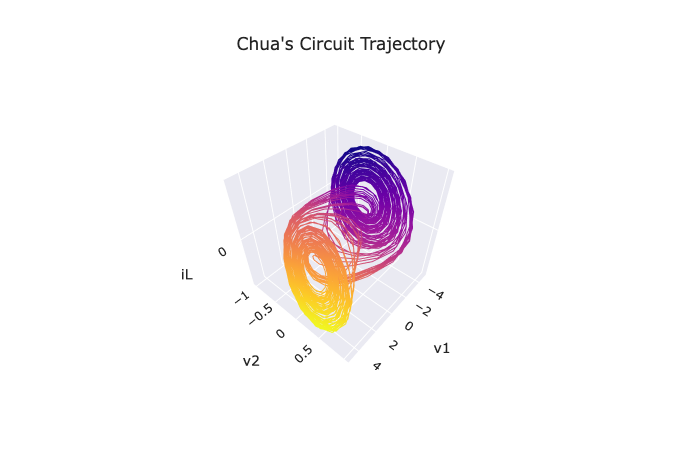
\includegraphics[width=0.7\textwidth]{./img/plots/3d_double_scroll.png}
                        \caption{3D Double Scroll Attractor - V1 vs V2 vs iL. In the figure, we have the 3D plot of the voltage on the capacitor 1 
                        versus the voltage on the capacitor 2 versus the current on the inductor. This graph was created using the deterministic chaos equations, as shown above.}
                        \label{fig: 3D Double Scroll Attractor - V1 vs V2 vs iL.}
                \end{figure} \pagebreak
                \begin{figure}[!htb]
                        \centering
                        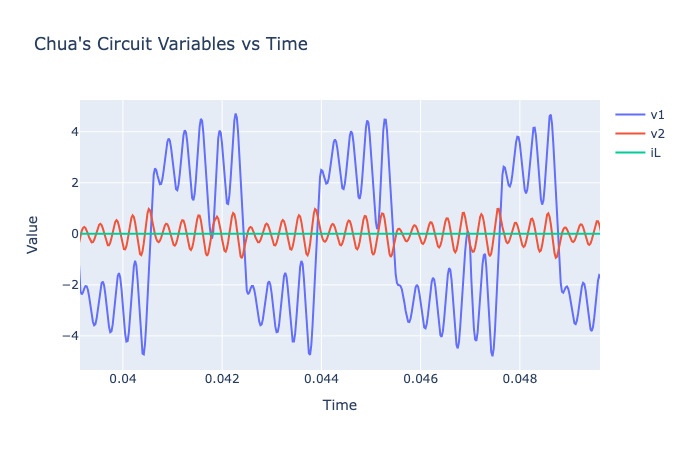
\includegraphics[width=0.7\textwidth]{./img/plots/Chua_Circuit_Variables_vs_Time.png}
                        \caption{Trail 2 - V1 and V2 vs time. In the figure, we have the plot of the voltage on the capacitor 1 and the voltage on the capacitor 2 versus time. 
                        Here we can see the sinusoidal behavior of the system. }
                \end{figure}
        


                As we can see, our results are consistent with the theoretical projections of chaotic dynamics. 
                The behavior of the Chua's circuit is highly sensitive to initial conditions, and small changes in the potentiometers 
                can lead to large and unpredictable differences in the long-term behavior of the system. The presence of strange attractors 
                and fractal patterns in the behavior of the Chua's circuit highlights the complex and unpredictable behavior of the system. 
                Understanding chaotic dynamics and its applications is crucial in various scientific fields, and the study of Chua's circuit offers 
                valuable insights into the behavior of complex systems.


                \subsubsection{Applications in Science and Engineering}
                The study of chaotic systems, such as Chua's circuit, has important implications for various scientific and engineering fields.
                By understanding the behavior of chaotic systems, researchers can gain insights into the underlying principles of complex systems
                and develop mathematical models that capture their behavior. This knowledge can be applied to a wide range of fields, including
                physics, biology, economics, and weather forecasting.

                In physics, chaotic systems are used to study the behavior of complex physical systems, such as fluid dynamics, plasma physics, and
                quantum mechanics. By understanding the chaotic dynamics of these systems, researchers can gain insights into their underlying
                principles and develop mathematical models that capture their behavior.

                \subsubsection{Limitations and Errors}
                The only limitation was the presence of noise in the data, which made it difficult to identify the presence of strange attractors in some cases;
                and the limits on the analog to digital converter of the oscilloscope which caused blocky data in the graphs.

                However the uncertanties in the data were small, and the results were consistent with the theoretical projections of chaotic dynamics.




\section{Conclusion}
Overall, the experiment was successful in empirically confirming the theoretical projections of chaotic dynamics and exploring the boundaries of classical 
mechanics under high-energy conditions. The behavior of Chua's circuit was highly sensitive to initial conditions, and small changes in the potentiometers 
led to large and unpredictable differences in the long-term behavior of the system. The presence of strange attractors and fractal patterns in the behavior 
of the Chua's circuit highlighted the complex and unpredictable behavior of the system. The results were consistent with the theoretical projections 
of chaotic dynamics, and the experiment provided valuable insights into the behavior of complex systems. Understanding chaotic dynamics and its applications 
is crucial in various scientific fields, and the study of Chua's circuit offers valuable insights into the behavior of complex systems. The only limitation
was the presence of noise in the data, which made it difficult to identify the presence of strange attractors in some cases; and the limits on the analog to
digital converter of the oscilloscope which caused blocky data in the graphs. However, the uncertanties in the data were small, and the results were consistent
with the theoretical projections of chaotic dynamics.

\section{References}
    \begin{enumerate}
        \sloppy

        \item  T. Matsumoto. A chaotic attractor from Chua’s circuit. IEEE Trans. Circuits Sys., 31(12):1055–1058, 1984.
        \item  http://www.chuacircuits.com For more information on setup, examples, and matlab example code.
        \item L. O. Chua, C. W. Wu, A. Huang and Guo-Qun Zhong, "A universal circuit for studying and generating chaos. I. Routes to chaos," in IEEE Transactions on Circuits and Systems I: Fundamental Theory and Applications, vol. 40, no. 10, pp. 732-744, Oct. 1993, doi: 10.1109/81.246149.
        \item Jihua Yang, Liqin Zhao,
        Bifurcation analysis and chaos control of the modified Chua’s circuit system,
        Chaos, Solitons and Fractals,
        Volume 77,
        2015,
        Pages 332-339,
        ISSN 0960-0779,
        https://doi.org/10.1016/j.chaos.2015.05.028.
        (https://www.sciencedirect.com/science/article/pii/S0960077915001642)

        

    \end{enumerate}

\end{document}
